% !TEX root = ../Zobkov_43501_3.tex
\section{Цель работы}

Ознакомление с заданными протоколами по RFC и их реализация.

\section{Программа работы}

\begin{enumerate}
	\item Ознакомление со протоколом (по RFC), определение набора необходимых команд для реализации;
	\item Создание базовой версии клиентского приложения/прокси, тестирование и отладка;
	\item Разработка GUI для клиентского приложения;
	\item Изучение средств взаимодействия GUI с потоками;
	\item Создание клиентского приложения с GUI, тестирование и отладка.
\end{enumerate}

\section{Индивидуальное задание}
\subsection{Прокси POP3} \label{proxy}

\paragraph{Задание:} 

разработать сервер-посредник для протокола POP3, функционирующий под управлением операционных систем Windows или Linux.

\paragraph{Основные возможности приложения:}

\begin{enumerate}
	\item Подключение нескольких почтовых клиентов;
	\item Разбор аутентификационных данных и получение имени POP3-сервера;
	\item Трансляция команд от клиента к серверу и обратно;
	\item Протоколирование обмена между почтовым клиентом и сервером.
\end{enumerate}

\paragraph{Поддерживаемые команды.} 

Разработанное приложение должно реализовывать следующие команды протокола POP3:

\begin{itemize}
	\item USER --– получение от клиента идентификационных данных пользователя вместе с адресом реального сервера;
	\item PASS --– получение от клиента пароля пользователя;
	\item STAT --– отправка клиенту состояния почтового ящика;
	\item LIST --– отправка клиенту списка сообщения почтового ящика;
	\item RETR --– отправка клиенту текста сообщения;
	\item DELE --– пометка сообщения на удаление;
	\item TOP --- отправка клиенту первых нескольких строк сообщения;
	\item UIDL --- выдача уникального идентификатора сообщения;
	\item RSET --- сброс всех пометок на удаление сообщений;
	\item QUIT --- удаление всех помеченных сообщений и завершение сеанса.
\end{itemize}

\paragraph{Методика тестирования.} 

Для тестирования приложения используется стандартный клиент электронной почты, имеющийся в лаборатории (Mozilla Thunderbird, The Bat, MS Outlook Express). Параметры учетной записи настраиваются на сокет, используемый разработанным приложением.

В качестве почтового сервера можно использовать лабораторные POP3-серверы или бесплатные почтовые службы (например, \href{http://www.mail.ru}{www.mail.ru}, \href{http://www.yandex.ru}{www.yandex.ru} и т. п.). Спроектированный прокси-сервер проверяется на выполнение набора основных функций протокола POP3.

\subsubsection{Анализ протокола}

Основные команды протокола приведены в \vref{tab:pop3}. Необходимые команды и их функции описаны в техническом задании (см. \vref{proxy}).

\begin{table}[H]
	\centering
	\begin{tabular}{|M{1.5cm}|M{3cm}|M{4.5cm}|M{7.5cm}|}
		\hline Имя & Аргументы & Ограничения & Возможные ответы \\
		\hline USER & [имя] & --- & +OK name is a valid mailbox \newline -ERR never heard of mailbox name \\
		\hline PASS & [пароль] & Работает после успешной передачи имени почтового ящика & +OK maildrop locked and ready \newline -ERR invalid password \newline -ERR unable to lock maildrop \\
		\hline DELE & [сообщение] & Доступна после успешной аутентификации & +OK message deleted \newline -ERR no such message \\
		\hline LIST & [сообщение] & Доступна после успешной аутентификации & +OK scan listing follows \newline -ERR no such message \\
		\hline RETR & [сообщение] & Доступна после успешной аутентификации & +OK message follows \newline -ERR no such message \\
		\hline RSET & --- & Доступна после успешной аутентификации & +OK \\
		\hline STAT & --- & Доступна после успешной аутентификации & +OK [кол-во писем] [размер в октетах] \\
		\hline TOP & [сообщение] [количество строк] & Доступна после успешной аутентификации & +OK n octets \newline -ERR no such message \\
		\hline QUIT & --- & --- & +OK Bye \\ \hline
	\end{tabular}
	\caption{Команды протокола POP3}
	\label{tab:pop3}
\end{table}

Прокси-сервер --- сервер-посредник, позволяющий клиентам совершать косвенные запросы к сетевым службам. Сначала клиент подключается к прокси-серверу и запрашивает какой-либо ресурс (в данном случае --- электронные письма), расположенный на другом сервере. Затем прокси-сервер подключается к данному серверу и получает ресурс у него. В некоторых случаях запрос клиента или ответ сервера может быть модифицирован прокси-сервером. Прокси-сервер позволяет защитить клиента от некоторых сетевых атак и помогает сохранить его анонимность.

\subsubsection{Архитектура приложения}

Реализованное приложение состоит из трех классов: \textit{Main}, \textit{MainThread} и \textit{ProxyThread}.

Класс \textit{Main} создает поток класса \textit{MainThread}. \textit{MainThread} реализует мультипоточный сервер с возможностью отображать список подключенных клиентов, принудительного отключения клиентов и отключения самого прокси-сервера, а также создание для каждого клиента потока класса \textit{ProxyThread} для выполнения основного функционала прокси-сервера.

Класс \textit{ProxyThread} получает из команды USER email пользователя, из которого извлекается целевой домен, к которому прокси-сервер подключается по SSL-соединению. После этого прокси-сервер переходит в штатный режим: пересылает команды от клиента к серверу и ответы сервера клиенту с протоколированием обмена.

\subsubsection{Тестирование}

Тестирование прокси-сервера проводилось с помощью клиента электронной почты Mozilla Thunderbird и адресов электронной почты доменов yandex.ru, gmail.com и mail.ru.

Пример настройки Thunderbird для работы с прокси-сервером представлен на \vref{pic:popsettings}.

\begin{figure}[H]
	\centering
	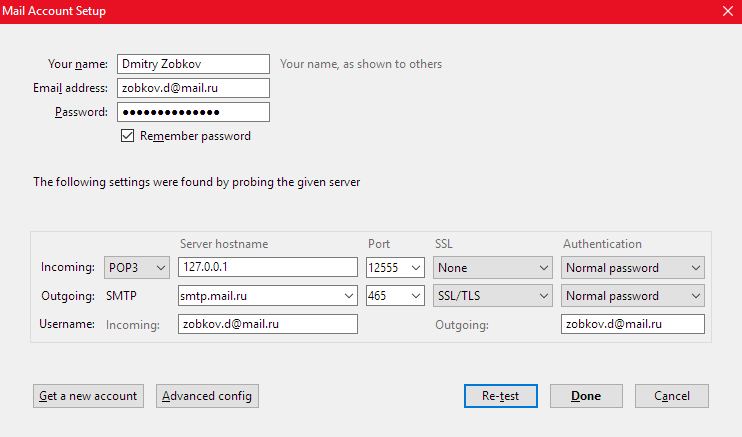
\includegraphics[width=0.8\textwidth]{popsettings}
	\caption{Настройка Thunderbird для работы с прокси-сервером}
	\label{pic:popsettings}
\end{figure}

Протокол подключения к почтовому серверу через прокси представлен в стандартном потоке вывода (листинг \vref{popconnect}).

\begin{lstlisting}[label=popconnect,caption=Результат подключения к серверу]
New connection: 127.0.0.1:55005
127.0.0.1:55005	client -> AUTH
-ERR What?
127.0.0.1:55005	client -> CAPA
+OK Capability list follows
USER
.
127.0.0.1:55005	client -> USER zobkov.d@mail.ru
Connected to pop.mail.ru:995
pop.mail.ru:995	server -> +OK

127.0.0.1:55005	client -> PASS **********
pop.mail.ru:995	server -> +OK Welcome!

127.0.0.1:55005	client -> QUIT
pop.mail.ru:995	server -> +OK POP3 server at mail.ru signing off

Disconnected: 127.0.0.1:55005 (Socket closed)
Socket closed.
\end{lstlisting}

Попытка получения всех писем с почтового ящика представлена в листинге \vref{poplist} (для краткости приводятся только первые 5 сообщений).

\begin{lstlisting}[label=poplist,caption=Получение всех сообщений (вывод сокращен до 5 сообщений)]
New connection: 127.0.0.1:55180
127.0.0.1:55180	client -> AUTH
-ERR What?
127.0.0.1:55180	client -> CAPA
+OK Capability list follows
USER
.
127.0.0.1:55180	client -> USER zobkov.d@mail.ru
Connected to pop.mail.ru:995
pop.mail.ru:995	server -> +OK

127.0.0.1:55180	client -> PASS **********
pop.mail.ru:995	server -> +OK Welcome!

127.0.0.1:55180	client -> STAT
pop.mail.ru:995	server -> +OK 67 4069642

127.0.0.1:55180	client -> LIST
pop.mail.ru:995	server -> +OK 67 messages (4069642 octets)
1 9811
2 8537
3 8537
4 47758
5 10388
.

127.0.0.1:55180	client -> UIDL
pop.mail.ru:995	server -> +OK 67 messages (4069642 octets)
1 145392614473
2 1456503272707
3 1456505765206
4 1464150824129
5 1465206601280
.

127.0.0.1:55180	client -> RETR 1
pop.mail.ru:995	server -> +OK 9811 octets <...>
127.0.0.1:55180	client -> RETR 2
pop.mail.ru:995	server -> +OK 8537 octets <...>
127.0.0.1:55180	client -> RETR 3
pop.mail.ru:995	server -> +OK 8537 octets <...>
127.0.0.1:55180	client -> RETR 4
pop.mail.ru:995	server -> +OK 47758 octets <...>
127.0.0.1:55180	client -> RETR 5
pop.mail.ru:995	server -> +OK 10388 octets <...>
127.0.0.1:55180	client -> QUIT
pop.mail.ru:995	server -> +OK POP3 server at mail.ru signing off

Disconnected: 127.0.0.1:55180 (Socket closed)
Socket closed.
\end{lstlisting}

Пример полученного сообщения представлен на \vref{pic:popmail}.

\begin{figure}[H]
	\centering
	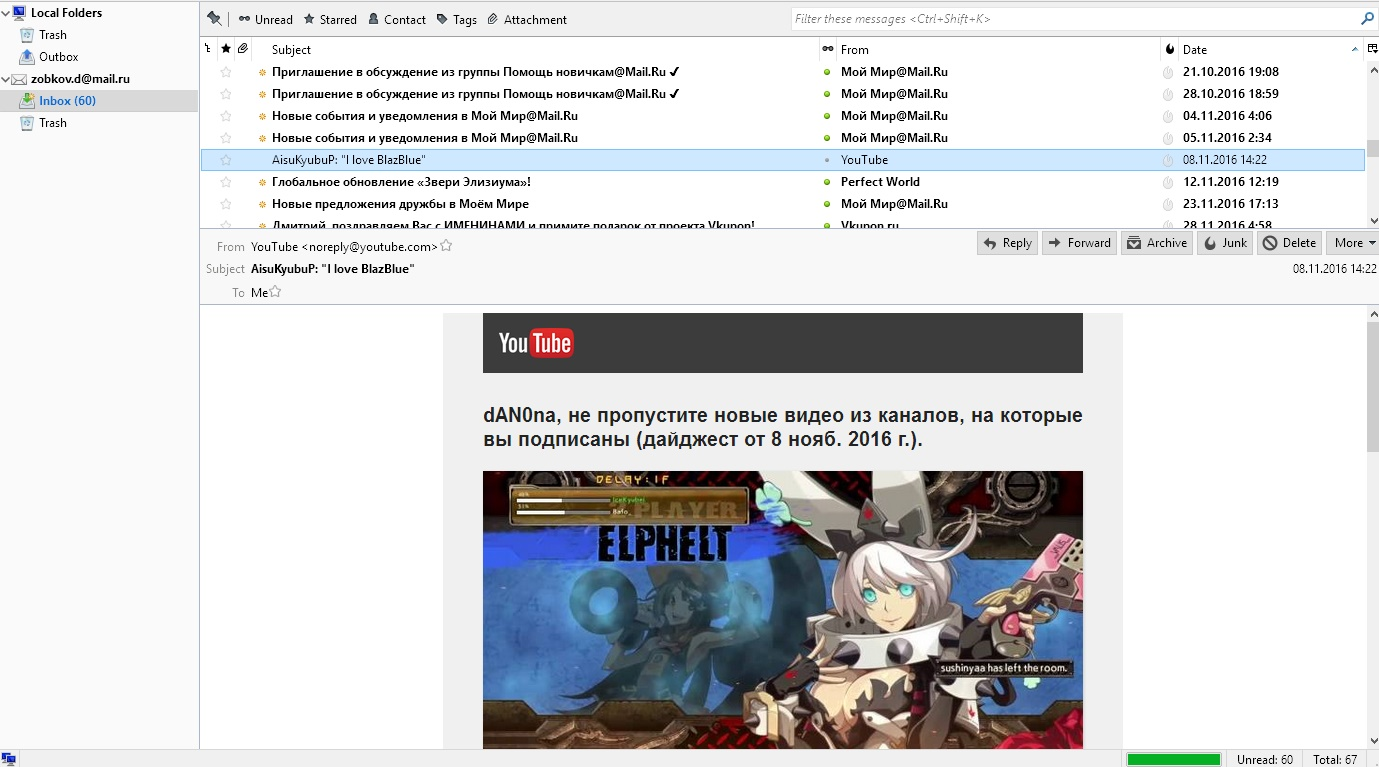
\includegraphics[width=\textwidth]{popmail}
	\caption{Пример полученного сообщения}
	\label{pic:popmail}
\end{figure}

Попытка удаления сообщения приведена в листинге \vref{popdele} и на \vref{pic:popdelete}.

\begin{lstlisting}[label=popdele,caption=Удаление сообщения]
127.0.0.1:55712	client -> DELE 37
pop.mail.ru:995	server -> +OK message 37 deleted
\end{lstlisting}

\begin{figure}[H]
	\centering
	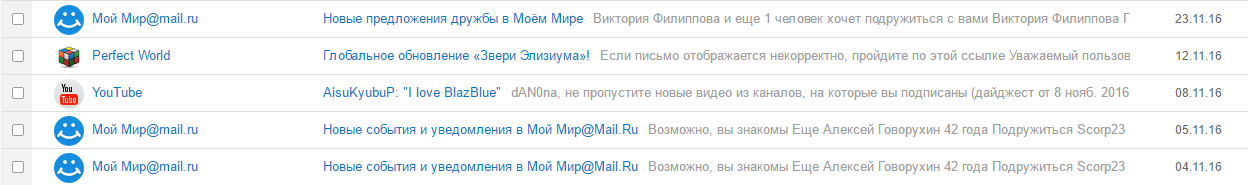
\includegraphics[width=\textwidth]{before}
	\\[0.5cm]
	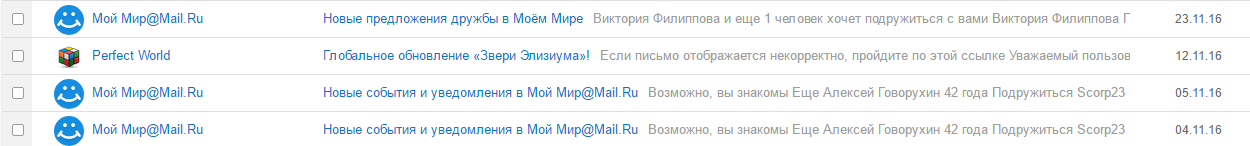
\includegraphics[width=\textwidth]{after}
	\caption{Удаление сообщения на сервере (до и после)}
	\label{pic:popdelete}
\end{figure}

Аналогичным образом были протестированы оставшиеся команды, требуемые по заданию. Также была проверена возможность подключения нескольких клиентов к разным серверам и их параллельная работа и продемонстрирована преподавателю.

\subsection{FTP клиент (пассивный режим работы)}

\paragraph{Задание:}

Разработать приложение для операционных систем семейства Windows или Linux, обеспечивающее функции клиента протокола FTP.

\paragraph{Основные возможности:}

Приложение должно реализовывать следующие функции:

\begin{enumerate}
	\item Подключение к указанному серверу;
	\item Получение списка файлов в каталоге;
	\item Навигация по системе каталогов;
	\item Копирование файла на сервер;
	\item Копирование файла с сервера;
	\item Создание и удаление каталогов;
	\item Удаление файлов;
	\item Обеспечение работы со ссылками на файлы и каталоги;
	\item Протоколирование соединения сервера с клиентом.
\end{enumerate}

\paragraph{Поддерживаемые команды.}

Разработанное приложение должно реализовывать следующие команды протокола FTP:

\begin{itemize}
	\item USER --- передача серверу идентификационной информации пользователя;
	\item PASS --- передача серверу пароля пользователя;
	\item CWD --- смена текущего каталога сервера;
	\item MKD --- создание каталога;
	\item RMD --- удаление каталога;
	\item DELE --- удаление файла на сервере;
	\item PASV --- переключение сервера в пассивный режим;
	\item LIST --- получение списка файлов в текущем каталоге сервера в расширенном формате;
	\item NLST --- получение списка файлов в текущем каталоге сервера в сокращенном формате;
	\item RETR --- получение файла с сервера;
	\item STOR --- посылка файла на сервер;
	\item QUIT --- завершение сеанса.
\end{itemize}

\paragraph{Настройки приложения.}

Разработанное приложение должно обеспечивать настройку следующих параметров:

\begin{enumerate}
	\item IP-адрес или доменное имя файлового сервера;
	\item Имя пользователя;
	\item Пароль пользователя.
\end{enumerate}

\paragraph{Методика тестирования.}

Для тестирования приложения следует использовать файловые серверы, имеющиеся в лаборатории, а также открытые файловые серверы, имеющиеся в сети Internet (\href{ftp://ftp.funet.fi}{ftp://ftp.funet.fi}, \href{ftp://ftp.relcom.ru}{ftp://ftp.relcom.ru} и т.п.).

Для разработанных приложений проверяется возможности подсоединения к серверу, копирования файла на сервер, копирования файла с сервера, удаления файла на сервере, переименовании файла на сервере, создания каталога, удаления каталога.

\subsubsection{Анализ протокола}

Команды протокола FTP, реализованные в клиенте, приведены на \vref{tab:ftp}.

\begin{table}[H]
	\centering
	\begin{tabular}{|M{1.5cm}|M{5cm}|M{10cm}|}
		\hline Имя & Аргументы & Описание \\
		\hline USER & [имя] & Имя пользователя \\
		\hline PASS & [пароль] & Пароль пользователя  \\
		\hline PWD & --- & Вывод текущей директории \\
		\hline CWD & [директория] & Смена директории \\
		\hline MKD & [имя] & Создание новой директории  \\
		\hline RMD & [директория] & Удаление директории  \\
		\hline DELE & [имя файла] & Удаление файла \\
		\hline PASV & --- & Перевод сервера в пассивный режим и получение IP и порта для получения данных \\
		\hline LIST & --- или [директория] & Список файлов и директорий в стиле UNIX-команды ls -l \\
		\hline NLST & [сообщение] & Аналогично LIST, но вывод в сокращенном формате --- только имена файлов/директорий  \\
		\hline RETR & [имя файла] & Скачать указанный файл  \\
		\hline STOR & [имя файла] & Загрузить файл на сервер  \\
		\hline SYST & --- & Возвращает тип системы сервера  \\
		\hline TYPE & [тип] & Выбор режима передачи  \\
		\hline SIZE & [имя файла] & Возвращает размер файла \\
		\hline QUIT & --- & Отключение  \\ \hline
	\end{tabular}
	\caption{Команды протокола FTP}
	\label{tab:ftp}
\end{table}

Сервер отвечает на команды клиента трехзначными кодами.

Первая цифра отвечает за один из трёх исходов: успех, отказ или указание на ошибку либо неполный ответ.

\begin{itemize}
	\item 2xx --- Успешный ответ;
	\item 4xx/5xx --- Команда не может быть выполнена;
	\item 1xx/3xx --- Ошибка или неполный ответ.
\end{itemize}

Вторая цифра определяет тип ошибки:

\begin{itemize}
	\item x0z --- Синтаксическая;
	\item x1z --- Информация. Соответствует информационному сообщению;
	\item x2z --- Соединения. Сообщение относится к управляющему соединению либо к соединению данных;
	\item x3z --- Соответствует сообщениям об аутентификации пользователя и его правах;
	\item x4z --- Не определено;
	\item x5z --- Файловая система. Соответствует сообщению о состоянии файловой системы.
\end{itemize}

Третья цифра окончательно специфицирует ошибку.

\subsubsection{Архитектура приложения}

Реализованное приложение состоит из четырех классов: \textit{Gui}, \textit{FTPClient}, \textit{FTPFile} и \textit{FTPResponse}.

Объект класса \textit{FTPFile} содержит информацию о имени, размере и типе (файл, директория или символическая ссылка) файла, полученного с помощью команды LIST.

Объект класса \textit{FTPResponse} содержит информацию о трехзначном коде ответа сервера и тексте сообщения, а также о наличии в ответе сервера разделителя "`--"' вместо пробела, сообщающего о наличии дополнительных строк ответа сервера с данным кодом.

Класс \textit{Gui} реализует графический интерфейс приложения с использованием библиотеки Swing.

Класс \textit{FTPClient} реализует основной функционал приложения: подключение к серверу с аутентификацией, обеспечение работы в пассивном режиме, выполнение команд и протоколирование команд и ответов сервера.

\subsubsection{Тестирование}

Внешний вид графического интерфейса представлен на \vref{pic:ftpgui}.

\begin{figure}[H]
	\centering
	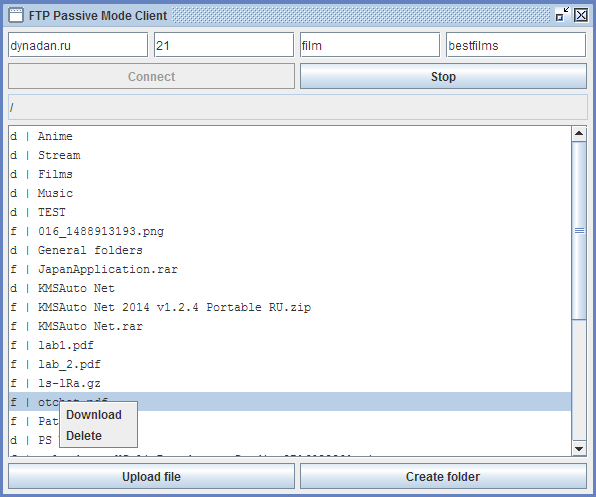
\includegraphics[width=0.8\textwidth]{ftpgui}
	\caption{Графический интерфейс}
	\label{pic:ftpgui}
\end{figure}

После подключения к FTP-серверу в стандартном потоке вывода отобразился процесс подключения (листинг \vref{connect}).

\begin{lstlisting}[label=connect,caption=Результат подключения к серверу]
<<< 220-FileZilla Server 0.9.55 beta
<<< 220-written by Tim Kosse (tim.kosse@filezilla-project.org)
<<< 220 Please visit https://filezilla-project.org/
>>> USER film
<<< 331 Password required for film
>>> PASS bestfilms
<<< 230 Logged on
>>> SYST
<<< 215 UNIX emulated by FileZilla
>>> PWD
<<< 257 "/" is current directory.
>>> TYPE I
<<< 200 Type set to I
>>> PASV
<<< 227 Entering Passive Mode (31,134,157,210,59,85)
<<< 31.134.157.210:15189
>>> LIST /
<<< 150 Opening data channel for directory listing of "/"
<<< 226 Successfully transferred "/"
\end{lstlisting}

Попытка перехода на другую директорию отражена в листинге \vref{cwd}.

\begin{lstlisting}[label=cwd,caption=Переход в папку тест]
>>> CWD TEST
<<< 250 CWD successful. "/TEST" is current directory.
>>> PWD
<<< 257 "/TEST" is current directory.
>>> SYST
<<< 215 UNIX emulated by FileZilla
>>> PWD
<<< 257 "/TEST" is current directory.
>>> TYPE I
<<< 200 Type set to I
>>> PASV
<<< 227 Entering Passive Mode (31,134,157,210,59,70)
<<< 31.134.157.210:15174
>>> LIST /TEST
<<< 150 Opening data channel for directory listing of "/TEST"
<<< 226 Successfully transferred "/TEST"
\end{lstlisting}

Аналогичным образом были протестированы все поддерживаемые команды (за исключением NLST и SIZE, т. к. они не используются графическим интерфейсом приложения, поэтому были протестированы при разработке). Также была проверена возможность параллельного скачивания и загрузки нескольких файлов большого размера и продемонстрирована преподавателю.

\section{Вывод}

В данных лабораторных работах были изучены средства создания клиентских/серверных сокетов TCP, средства записи/чтения из сокетов и средства многонитевой работы в Java. Были разработаны прокси POP3 и FTP-клиент с работой в пассивном режиме, для которого был создан графический интерфейс с использованием библиотеки Swing.

Разработанные приложения были протестированы в реальных условиях. Для тестирования POP3 прокси использовался почтовый клиент Mozilla Thunderbird и и адреса электронной почты доменов yandex.ru, gmail.com и mail.ru. Для тестирования FTP-клиента использовались как FTP-сервер, созданный в локальной сети, что позволило протестировать действия, требующие прав на выполнение (создание/удаление папок, загрузка/удаление файлов), так и открытые файловые серверы в сети Интернет.

В настоящее время существует множество сторонних библиотек, упрощающих разработку данных протоколов до нескольких строк. Например, с использованием библиотеки Apache можно значительно облегчить разработку POP3 и FTP клиентов. Также можно воспользоваться библиотекой Javamail для упрощенной разработки POP3 и IMAP клиентов.

Разработка сетевых приложений при использовании языка Java значительно упрощается по сравнению с разработкой на языках C/C++. Это вызвано упрощенной работой с сокетами, большим количеством существующих библиотек, меньшим количеством отслеживаемых ошибок.































































% \section{Цель работы}

% Получение навыков исследования сетевого трафика.

% \section{Программа работы}

% При помощи анализатора сетевого трафика WireShark продемонстрировать в сети работу следующих протоколов и утилит:

% \begin{enumerate}
% 	\item Утилиты ping:
% 	\begin{itemize}
% 		\item без фрагментации;
% 		\item с фрагментацией.
% 	\end{itemize}
% 	\item Утилиты tracert;
% 	\item Протокола ARP: запрос и ответ;
% 	\item Протокола ICMP: пронаблюдать ошибку типа 3;
% 	\item Протокола UDP: попытка отправления UDP-пакета на несуществующий порт. 
% 	\item Протокола TCP:
% 	\begin{itemize}
% 		\item установка соединения;
% 		\item разрыв соединения;
% 		\item попытка соединения на отсутствующий порт.
% 	\end{itemize}
% \end{enumerate}

% \section{Конфигурация сети} \label{sec:conf}

% Опыты проводились с использованием двух ПК, находящихся в одной сети (\vrefrange{pic:pc1}{pic:pc2}).

% \begin{figure}[H]
% 	\centering
% 	\includegraphics[width=\textwidth]{pc1}
% 	\caption{Конфигурация ПК 1}
% 	\label{pic:pc1}
% \end{figure}

% \begin{figure}[H]
% 	\centering
% 	\includegraphics[width=\textwidth]{pc22}
% 	\caption{Конфигурация ПК 2}
% 	\label{pic:pc2}
% \end{figure}

% \section{Ход работы}

% \subsection{Утилита ping}

% Утилита ping отправляет эхо-запрос ICMP, после чего в случае успеха должен прийти симметричный эхо-ответ ICMP. Если пакет не пришел за некоторое TTL, то удаленный сервер считается недостижимым. По умолчанию производится четыре попытки.

% \subsubsection{ping без фрагментации}

% Трафик утилиты Ping со стандартными параметрами bytes = 32, TTL = 128 (\vrefrange{pic:ping1}{pic:ping3}).

% \begin{figure}[H]
% 	\centering
% 	\includegraphics[width=0.7\textwidth]{ping1}
% 	\caption{Вызов утилиты в командной строке}
% 	\label{pic:ping1}
% \end{figure}

% \begin{figure}[H]
% 	\centering
% 	\includegraphics[width=\textwidth]{ping2}
% 	\caption{ICMP эхо-запрос}
% 	\label{pic:ping2}
% \end{figure}

% \begin{figure}[H]
% 	\centering
% 	\includegraphics[width=\textwidth]{ping3}
% 	\caption{ICMP эхо-ответ}
% 	\label{pic:ping3}
% \end{figure}

% Пакеты были распознаны как ICMP с пометкой "`Echo (ping) reply/request"'. Тип сообщения 8 соответствует эхо-запросу, а тип 0 --- эхо-ответу. Графа \textit{Destination} показывает IP-адрес назначения посылаемого пакета, а \textit{Source} --- IP-адрес источника. В качестве передаваемой информации используются коды символов a-w.

% \subsubsection{ping с фрагментацией}

% Для фрагментации пакета необходимо указать его размер, превышающий MTU (maximum transmission unit) --- максимальный размер полезного блока данных одного пакета, который может быть передан протоколом без фрагментации. Максимальный размер одного блока данных, который может быть передан без фрагментации составляет 1480 байт. 

% С помощью утилиты ping изменим размер буфера отправки на 8192 байта (\vref{pic:ping21}).

% \begin{figure}[H]
% 	\centering
% 	\includegraphics[width=\textwidth]{ping21}
% 	\caption{Вызов утилиты в командной строке}
% 	\label{pic:ping21}
% \end{figure}

% О фрагментированности пакета свидетельствуют флаги пакета IP (0x01 --- имеются еще фрагменты). О том, что это первый пакет из фрагментированных, свидетельствует нулевое смещение фрагмента (\vref{pic:ping22}). Каждый следующий пакет имеет frament offset увеличенный на 1480 по сравнению с предыдущим.

% Также можно заметить, что первый пакет был отправлен по протоколу ICMP, содержит заголовок ICMP (8 байт) и данные (1472 байта), а следующие фрагментированные пакеты передавались по протоколу IPv4 уже без заголовка ICMP.

% \begin{figure}[H]
% 	\centering
% 	\includegraphics[width=0.9\textwidth]{ping1new}
% 	\caption{Первый фрагмент пакета ping-запроса}
% 	\label{pic:ping22}
% \end{figure}

% Второй пакет все так же имеет флаг в заголовке IP-пакета (0x01), свидетельствующий о наличии пакетов кроме данного. От первого пакета его отличает ненулевое смещение фрагмента (\vref{pic:ping23}).

% \begin{figure}[H]
% 	\centering
% 	\includegraphics[width=\textwidth]{ping2new}
% 	\caption{Второй фрагмент пакета ping-запроса}
% 	\label{pic:ping23}
% \end{figure}

% Пакет, содержащий последний фрагмент ping-запроса, уже не имеет флагов в заголовке IP-пакета. При этом смещение фрагмента ненулевое, а идентификатор совпадает с идентификаторами пакетов, отправленных ранее (\vref{pic:ping24}).

% \begin{figure}[H]
% 	\centering
% 	\includegraphics[width=\textwidth]{ping3new}
% 	\caption{Последний фрагмент пакета ping-запроса}
% 	\label{pic:ping24}
% \end{figure}

% \subsection{Утилита tracert}

% Пронаблюдаем трассировку маршрута пакетов до узла \texttt{ya.ru} при помощи протокола ICMP и утилиты tracert (\vref{pic:trace1}).

% \begin{figure}[H]
% 	\centering
% 	\includegraphics[width=\textwidth]{trace1}
% 	\caption{Результат трассировки маршрута в консоли}
% 	\label{pic:trace1}
% \end{figure}

% Первый пакет трассировки маршрута отправляется с TTL равным 1. Это значит, что на первом же маршрутизаторе пакет будет уничтожен и нам придет сообщение об ошибке (\vrefrange{pic:tracert1}{pic:trace2}).

% \begin{figure}[H]
% 	\centering
% 	\includegraphics[width=\textwidth]{tracert1}
% 	\caption{Отправка первого пакета трассировки}
% 	\label{pic:tracert1}
% \end{figure}

% \begin{figure}[H]
% 	\centering
% 	\includegraphics[width=\textwidth]{trace2}
% 	\caption{Ответ на первый пакет трассировки}
% 	\label{pic:trace2}
% \end{figure}

% В сообщении об ошибке указан тип ICMP-пакета – 11.0, что означает, что время жизни пакета истекло. Сообщение пришло от маршрутизатора сети, который имеет адрес 192.168.0.1.  При ответе в пакете также пристыковывается IP-заголовок запроса.

% \begin{figure}[H]
% 	\centering
% 	\includegraphics[width=\textwidth]{trace3}
% 	\caption{Второй пакет трассировки маршрута}
% 	\label{pic:trace3}
% \end{figure}

% Следующий пакет будет отправлен на тот же адрес, что и ранее, но параметр TTL будет установлен в 2, чтобы пройти маршрутизатор по адресу 192.168.0.1 и попасть в следующий пункт передачи (\vref{pic:trace3}).

% \begin{figure}[H]
% 	\centering
% 	\includegraphics[width=\textwidth]{trace4}
% 	\caption{Ответ на второй пакет трассировки}
% 	\label{pic:trace4}
% \end{figure}

% В ответе на второй пакет трассировки маршрута в качестве отправителя сообщения об ошибке истечения жизни пакета указан адрес 10.145.138.1 (\vref{pic:trace4}). Значит, это и есть следующий пункт передачи. 

% Аналогично продолжается трассировка маршрута дальше с постепенным инкрементом параметра TTL. Таким образом составляется примерный маршрут прохождения IP-пакета до узла с адресом \texttt{www.yandex.ru}.


% \subsection{Протокол ARP}

% Рассмотрим пару APR пакетов, демонстрирующую работу протокола (\vrefrange{pic:arp1}{pic:arp2}).

% \begin{figure}[H]
% 	\centering
% 	\includegraphics[width=\textwidth]{arp1new}
% 	\caption{ARP-запрос}
% 	\label{pic:arp1}
% \end{figure}

% Был отправлен широковещательный ARP-запрос. В пакете ARP указывается его тип (поле Opcode) --– 0x1 для запроса и 0x2 для ответа. Указан целевой IP-адрес, для которого запрашивается MAC-адрес, целевой MAC-адрес при этом обнулен.

% \begin{figure}[H]
% 	\centering
% 	\includegraphics[width=\textwidth]{arp2new}
% 	\caption{ARP-ответ}
% 	\label{pic:arp2}
% \end{figure}

% В ответе возвращается результирующий MAC-адрес.

% % При попытке отправить ICMP эхо-запрос на несуществующий адрес (192.168.0.70), роутер начал посылать широковещательные ARP-запросы для идентификации неизвестного для него адреса в сети (\vref{pic:arp3}).

% % \begin{figure}[H]
% % 	\centering
% % 	\includegraphics[width=\textwidth]{arp3}
% % 	\caption{Широковещательный ARP-запрос}
% % 	\label{pic:arp3}
% % \end{figure}

% \subsection{Протокол ICMP}

% Для того, чтобы пронаблюдать ошибку типа 3.1 (целевой узел недостижим), отправим ping запрос на несуществующий адрес 192.168.0.70 (\vref{pic:icmp1}).

% \begin{figure}[H]
% 	\centering
% 	\includegraphics[width=0.7\textwidth]{icmp1}
% 	\caption{Вызов утилиты в командной строке}
% 	\label{pic:icmp1}
% \end{figure}

% В пакете можно наблюдать типичный ping-запрос --- ICMP-пакет типа 8.0 (\vref{pic:icmp2}).

% \begin{figure}[H]
% 	\centering
% 	\includegraphics[width=\textwidth]{icmp2}
% 	\caption{ICMP эхо-запрос}
% 	\label{pic:icmp2}
% \end{figure}

% Ответом на указанный выше запрос будет ICMP-пакет типа 3.1, свидетельствующий об ошибке "`целевой узел недостижим"' (\vref{pic:icmp3}). Также ответ содержит данные, которые были посланы при запросе (пристыкованный IP-заголовок).

% \begin{figure}[H]
% 	\centering
% 	\includegraphics[width=\textwidth]{icmp3}
% 	\caption{ICMP-ответ}
% 	\label{pic:icmp3}
% \end{figure}

% За ICMP-пакетом типа 3.1 следует ICMP-пакет типа 5.1 --- Redirect datagrams for the Host (\vref{pic:icmp4}).
% % Данный пакет сообщает хосту о необходимости создания нового маршрута к указанному в сообщении хосту и внесения его в таблицу маршрутизации. В сообщении указывается IP адрес хоста, где необходима смена маршрута (адрес занесен в поле Destination в пристыкованном IP заголовке), и новый IP адрес маршрутизатора, на который необходимо направлять пакеты, адресованные данному хосту (этот адрес заносится в поле Gateway).
% Этот пакет формируется в том случае, когда при получении дейтаграммы шлюз обнаруживает, что для ее передачи был выбран неудачный маршрут. Таким пакетом шлюз рекомендует хосту (адрес в поле Destination в пристыкованном IP заголовке) впредь отправлять отправлять дейтаграммы через шлюз, указанный в поле Gateway address (в нашем случае, напрямую на недостижимый узел --- 192.168.0.70).

% % Gateway адрес по прежнему остался недостижимым узлом 192.168.0.70.

% \begin{figure}[H]
% 	\centering
% 	\includegraphics[width=\textwidth]{icmp4}
% 	\caption{Пакет перенаправления}
% 	\label{pic:icmp4}
% \end{figure}

% \subsection{Протокол UDP}

% Для отправки UDP-пакета на непрослушиваемый порт была написана соответствующая программа (\Vref{app:udp}).

% \begin{figure}[H]
% 	\centering
% 	\includegraphics[width=\textwidth]{udp1}
% 	\caption{UDP-пакет}
% 	\label{pic:udp}
% \end{figure}

% UDP-пакет был отправлен на непрослушиваемый порт 8005, в качестве пересылаемых данных выступали 5 байт текста --- dAN0n.

% В ответ был получен ICMP-ответ с ошибкой типа 3.3 (порт недостижим). Также ответ содержит данные, которые были посланы при запросе (пристыкованный IP-заголовок).

% \begin{figure}[H]
% 	\centering
% 	\includegraphics[width=\textwidth]{udp2}
% 	\caption{ICMP-ответ}
% 	\label{pic:udp2}
% \end{figure}

% \subsection{Протокол TCP}

% Все последующие опыты были выполнены при использовании двух ПК, находящихся в одной сети. Их сетевые параметры представлены в \vref{sec:conf}. Были написаны программы TCP сервера и клиента (\Vrefrange{app:server}{app:client}). На одном из ПК будет запущен TCP-сервер, а на другом TCP-клиент.

% \subsubsection{Установка соединения}

% При установке соединения между клиентом и сервером происходит передача трех пакетов. Клиент посылает серверу сегмент с номером последовательности и флагом SYN (\vref{pic:tcp1}).

% \begin{figure}[H]
% 	\centering
% 	\includegraphics[width=\textwidth]{tcp1}
% 	\caption{Первый пакет при установке TCP-соединения}
% 	\label{pic:tcp1}
% \end{figure}

% В случае успеха сервер посылает клиенту сегмент с номером последовательности и флагами SYN и ACK, и переходит в состояние SYN-RECEIVED (\vref{pic:tcp2}). В случае неудачи сервер посылает клиенту сегмент с флагом RST.

% \begin{figure}[H]
% 	\centering
% 	\includegraphics[width=\textwidth]{tcp2}
% 	\caption{Второй пакет при установке TCP-соединения}
% 	\label{pic:tcp2}
% \end{figure}

% В заголовке TCP-пакета также имеются:
% \begin{itemize}
% 	\item Sequence Number --- порядковый номер: 32 бита;
% 	\item Acknowledgment Number --- номер подтверждения: 32 бита.
% \end{itemize} ~\\

% "`Relative sequence/ack number"' говорит о том, что вместо использования реальных значений seq/ack number, Wireshark использует относительные значения для упрощения анализа (значения получаются меньше реальных, которые обычно генерируются случайным образом во время SYN фазы).

% В первом пакете относительный seq number: 0, ack number: 0. Так как это первый пакет для инициализации
% соединения, реальный seq number был сгенерирован случайным образом (например, $x$), а ack number равен 0, т.к. ответов от сервера еще поступало.

% Во втором пакете сервер сгенерировал свой реальный seq number (например, $y$), относительный seq number: 0, в поле же ack number записано 1 (реальный --- $x+1$), т.е. сервер инкрементировал полученный от клиента seq number, и теперь ожидает от него пакет с соответствующим seq number.

% Последний этап --- отправка на сервер пакета с установленным флагом ACK, после чего соединение переходит в состояние ESTABLISHED (\vref{pic:tcp3}).

% \begin{figure}[H]
% 	\centering
% 	\includegraphics[width=\textwidth]{tcp3}
% 	\caption{Третий пакет при установке TCP-соединения}
% 	\label{pic:tcp3}
% \end{figure}

% В третьем пакете, относительный seq number равен 1 (реальный --- $x+1$), а ack number равен 1 (реальный --- $y+1$), теперь клиент ожидает от сервера пакет с seq number равным 1 (реальным --- $y+1$).

% \subsubsection{Разрыв соединения}

% % При разрыве соединения сервер отсылает клиенту пакет с установленным флагом RST (\vref{pic:tcp21}).

% % \begin{figure}[H]
% % 	\centering
% % 	\includegraphics[width=\textwidth]{tcp21}
% % 	\caption{Пример пакета с флагом RST}
% % 	\label{pic:tcp21}
% % \end{figure}

% Будет рассмотрен случай разрыва соединения со стороны клиента.

% % Если соединение уже было установлено, то завершение соединения со стороны клиента производится следующим образом:

% Клиент посылает серверу пакет с установленными флагами [FIN, ACK]. Клиент переходит из состояния
% ESTABLISHED в состояние FIN-WAIT-1 (\vref{pic:tcp1new}).

% \begin{figure}[H]
% 	\centering
% 	\includegraphics[width=\textwidth]{tcp1new}
% 	\caption{Первый пакет от клиента}
% 	\label{pic:tcp1new}
% \end{figure}

% Сервер при получении пакета переходит из состояния ESTABLISHED в состояние CLOSE-WAIT. И посылает
% в ответ два пакета. Первый пакет содержит флаг [ACK], после принятия пакета клиентом, он переходит в
% состояние FIN-WAIT-2 (\vref{pic:tcp2new}).

% \begin{figure}[H]
% 	\centering
% 	\includegraphics[width=\textwidth]{tcp2new}
% 	\caption{Первый пакет от сервера}
% 	\label{pic:tcp2new}
% \end{figure}

% Сервер посылает второй пакет с флагами [FIN, ACK], после его отсылки сервер переходит в состояние
% LAST-ACK, а клиент в состояние TIME-WAIT (\vref{pic:tcp3new}).

% \begin{figure}[H]
% 	\centering
% 	\includegraphics[width=\textwidth]{tcp3new}
% 	\caption{Второй пакет от сервера}
% 	\label{pic:tcp3new}
% \end{figure}

% Клиент посылает серверу пакет с флагом [ACK], и переходит в состояние CLOSED для данного соединения.
% Сервер так-же при принятии пакета переходит в состояние CLOSED (\vref{pic:tcp4new}).

% \begin{figure}[H]
% 	\centering
% 	\includegraphics[width=\textwidth]{tcp4new}
% 	\caption{Второй пакет от клиента}
% 	\label{pic:tcp4new}
% \end{figure}

% \subsubsection{Попытка соединения на отсутствующий порт}

% При попытке подключения к отсутствующему порту, от адреса, к которому происходит подключение, приходят пакеты с флагами ACK и RST. После трех попыток соединения, написанная программа (для удобства написанная для Windows, см. \Vref{app:port}) сообщает об ошибке.

% \begin{figure}[H]
% 	\centering
% 	\includegraphics[width=\textwidth]{tcp33}
% 	\caption{Попытка TCP-соединения c 192.168.0.25:8006}
% 	\label{pic:tcp31}
% \end{figure}

% \section{Вывод}

% В ходе работы был исследован сетевой трафик утилит ping и tracert, а также протоколов ICMP, ARP, TCP и UDP.

% При выполнении работы были рассмотрены различные ситуации, возникающие во время функционирования сети, такие как:

% \begin{itemize}
% 	\item Работа ICMP протокола при использовании утилиты ping (включая случай с фрагментацией);
% 	\item Работа ICMP протокола при использовании утилиты tracert;
% 	\item Работа ICMP протокола при возникновении ошибки 3.1 (Destination host unreachable);
% 	\item Работа TCP протокола при установке/разрыве соединения, а также попытке соединения с отсутствующим портом;
% \end{itemize}

% Для различных ситуаций использование программ анализа сетевого трафика позволяет более подробно рассмотреть происходящие при этом события.
